\chapter[Ihara Zeta Functions, Ramanujan Graphs and Hitting Times]{Ihara Zeta Functions,\\ Ramanujan Graphs and Hitting Times}\label{ch:08}

In 1966 Ihara attached to a discrete, torsion free, cocompact subgroup $\Gamma$ of $\PGL_2$ over a $p$ adic field with residue field of order $q$ a zeta function, an Euler product over the primitive closed geodesics of the finite quotient graph $\Gamma\backslash\T_q$, and proved that it is a rational function whose poles are governed by the eigenvalues of the Hecke operator \cite{ihara1966}. Sunada, Hashimoto and Bass later recognised that the construction makes sense for any finite graph \cite{sunada1986,hashimoto1989,bass1992}. For a regular graph the analogue of the Riemann hypothesis is a statement about eigenvalues that Lubotzky, Phillips and Sarnak, motivated by the Ramanujan conjecture, called the Ramanujan property \cite{lps1988}. We read the graph Riemann hypothesis three ways: as a statement about poles, about eigenvalues and about how fast a random walk forgets its start. We then turn to supersingular isogeny graphs, whose spectra are Hecke eigenvalues, and prove that their Kemeny constant, the expected time to hit a uniformly random target, is asymptotic to $\ell/(\ell-1)$ times the number of vertices.

\section{The Ihara zeta function}\index{Ihara zeta function}

Let $G$ be a finite connected graph, possibly with loops and multiple edges, with vertex set $V$, $n=|V|$, and edge set $E$. Orient each edge both ways, and let $A(x,y)$ count the oriented edges from $x$ to $y$, so that a loop contributes $2$ to the diagonal of the adjacency matrix $A$. A closed path $C=(e_1,\dots,e_m)$ of oriented edges is \emph{reduced} if $e_{i+1}\ne\bar e_i$ for all $i$ (indices mod $m$, so there is no backtracking and no tail), and \emph{primitive} if it is not a power $D^k$ with $k\ge2$. A \emph{prime} $\mathfrak p$ is an equivalence class of primitive reduced closed paths under cyclic rotation; its length is $\nu(\mathfrak p)$. The Ihara zeta function is
\[
Z_G(u)=\prod_{\mathfrak p}\bigl(1-u^{\nu(\mathfrak p)}\bigr)^{-1},
\]
convergent for small $|u|$. Then $u\,Z_G'(u)/Z_G(u)=\sum_{m\ge1}N_mu^m$, where $N_m$ counts reduced closed paths of length $m$: $Z_G$ counts closed nonbacktracking walks as $\zeta$ counts prime powers.

\begin{theorem}[Ihara \cite{ihara1966}; Bass \cite{bass1992}; Hashimoto \cite{hashimoto1989}]
If $G$ is $(q+1)$ regular with adjacency matrix $A$, then
\[
Z_G(u)^{-1}=(1-u^2)^{r-1}\det\bigl(I-Au+qu^2I\bigr),
\]
where $r=|E|-n+1$ is the rank of the fundamental group of $G$, so that $r-1=(q-1)n/2$.
\end{theorem}

The proof writes $N_m=\tr H^m$, where $H$ is the nonbacktracking (Hashimoto) matrix indexed by the $2|E|$ oriented edges, so that $Z_G(u)^{-1}=\det(I-uH)$, and evaluates this determinant by a block matrix identity equivalent to the recursions for $A_m$ in Theorem~\ref{thm:07tree}. For each eigenvalue $\lambda$ of $A$ the factor $1-\lambda u+qu^2$ contributes two poles $u_\pm$ with $u_+u_-=1/q$ and $u_++u_-=\lambda/q$. For $q\ge2$ the factor $(1-u^2)^{r-1}$ contributes poles at $u=\pm1$; the eigenvalue $\lambda=q+1$ gives poles at $u=1$ and $u=1/q$, and if $G$ is bipartite the eigenvalue $-(q+1)$ gives poles at $u=-1$ and $u=-1/q$. The poles in $\{\pm1,\pm1/q\}$ are the \emph{trivial} poles. In the variable $u=q^{-s}$ the pole at $u=1/q$ is $s=1$, and the circle $|u|=q^{-1/2}$ is the line $\Re s=\tfrac12$.

\begin{definition}\index{Ramanujan graph}
A $(q+1)$ regular graph satisfies the \emph{graph Riemann hypothesis} if every nontrivial pole of $Z_G$ lies on $|u|=q^{-1/2}$. It is \emph{Ramanujan} if every eigenvalue $\lambda$ of $A$ with $|\lambda|\ne q+1$ satisfies $|\lambda|\le2\sqrt q$.
\end{definition}

The name reflects the fact that for the graphs of Lubotzky, Phillips and Sarnak and for the isogeny graphs below the bound is the Ramanujan conjecture for weight two modular forms, which is a theorem: Eichler \cite{eichler1954} deduced it for prime level from Weil's Riemann hypothesis for curves over finite fields through the Eichler Shimura relation, and Deligne \cite{deligne1974} proved it in all weights. The bound $2\sqrt q$ is the edge of the support of the Kesten McKay law $\mu_q$ of Chapter~\ref{ch:07} after rescaling, and by the Alon Boppana theorem it cannot be improved for infinite families \cite{nilli1991}\index{Alon Boppana bound} (Exercise~\ref{ex:08alon} proves a weak form).

\section{Three forms of the Riemann hypothesis for graphs}

Let $P=A/(q+1)$ be the transition matrix of simple random walk on $G$; its stationary law is uniform. Order the eigenvalues of $A$ as $q+1=\lambda_1\ge\lambda_2\ge\dots\ge\lambda_n$, let $\mu_j=\lambda_j/(q+1)$, and define
\[
\lambda_*=\max\{|\lambda_j|:|\lambda_j|\ne q+1\},\qquad \delta_t=\max_{x\in V}\Bigl|P^t(x,x)-\frac{1+\beta(-1)^t}{n}\Bigr|,
\]
where $\beta=1$ if $G$ is bipartite and $\beta=0$ otherwise, and $\lambda_*=0$ if no eigenvalue has $|\lambda_j|\ne q+1$. Thus $\delta_t$ measures how far return probabilities are from their stationary (or, in the bipartite case, periodic stationary) values. Write $\rho_q=2\sqrt q/(q+1)$ for the Kesten rate of the tree (Chapter~\ref{ch:07}).

\begin{proposition}[this book]\label{prop:08three}\index{graph Riemann hypothesis}
For a connected $(q+1)$ regular graph $G$ the following are equivalent.
\begin{enumerate}
\item $Z_G$ satisfies the graph Riemann hypothesis.
\item $G$ is Ramanujan.
\item $\limsup_{t\to\infty}\delta_t^{1/t}\le\rho_q$.
\end{enumerate}
Moreover $\limsup_t\delta_t^{1/t}=\lambda_*/(q+1)$ exactly, so the return probabilities of a Ramanujan graph approach equilibrium at an exponential rate no slower than the rate $\rho_q$ at which the return probabilities of the tree tend to zero.
\end{proposition}

\begin{proof}
(1)$\Leftrightarrow$(2). By the Ihara Bass formula every pole of $Z_G$ is $\pm1$ or a root of $1-\lambda_ju+qu^2$ for some $j$, and every such root is a pole. If $|\lambda_j|\le2\sqrt q$ the discriminant $\lambda_j^2-4q$ is nonpositive, the roots are complex conjugates (or a double real root) and $|u_\pm|^2=u_+u_-=1/q$. If $2\sqrt q<|\lambda_j|<q+1$, the roots are real and distinct with product $1/q$, so one of them has modulus strictly less than $q^{-1/2}$; neither is trivial, since $\pm1$ or $\pm1/q$ is a root only when $\lambda_j=\pm(q+1)$. The eigenvalues $\pm(q+1)$ give only trivial poles. Hence all nontrivial poles lie on the circle if and only if every $\lambda_j$ with $|\lambda_j|\ne q+1$ satisfies $|\lambda_j|\le2\sqrt q$.

(2)$\Leftrightarrow$(3). Let $\phi_1,\dots,\phi_n$ be an orthonormal eigenbasis of $A$ in $\ell^2(V)$ with $\phi_1\equiv n^{-1/2}$. Then $P^t(x,x)=\sum_j\mu_j^t\phi_j(x)^2$ and $\sum_j\phi_j(x)^2=1$. Since $G$ is connected, $\lambda_1=q+1$ is simple, and $-(q+1)$ is an eigenvalue (then simple, with eigenvector $n^{-1/2}(\pm1)$ on the two sides) if and only if $G$ is bipartite. Removing these terms,
\[
P^t(x,x)-\frac{1+\beta(-1)^t}{n}=\sum_{j\in J}\mu_j^t\phi_j(x)^2,
\]
where $J$ indexes the eigenvalues with $|\lambda_j|\ne q+1$. The right side is bounded in absolute value by $(\lambda_*/(q+1))^t$, so $\limsup\delta_t^{1/t}\le\lambda_*/(q+1)$. Conversely, for even $t$ all terms are nonnegative, and averaging over $x$,
\[
\delta_t\ge\frac1n\sum_x\sum_{j\in J}\mu_j^t\phi_j(x)^2=\frac1n\sum_{j\in J}\mu_j^t\ge\frac1n\Bigl(\frac{\lambda_*}{q+1}\Bigr)^t,
\]
so $\limsup\delta_t^{1/t}\ge\lambda_*/(q+1)$. Hence the limsup equals $\lambda_*/(q+1)$, and it is at most $\rho_q=2\sqrt q/(q+1)$ if and only if $\lambda_*\le2\sqrt q$.
\end{proof}

The Riemann hypothesis for $Z_G$ is therefore a statement about mixing. Applied to off diagonal entries, the same argument gives the uniform bound $|P^t(x,y)-1/n|\le(\lambda_*/(q+1))^t$ in the nonbipartite case (Appendix~\ref{app:A}), so $\max_{x,y}|nP^t(x,y)-1|\le\varepsilon$ once $t\ge\log(n/\varepsilon)/\log((q+1)/\lambda_*)$.

\section{Supersingular isogeny graphs}\index{supersingular isogeny graph}

Let $N$ be a prime and $\ell\ne N$ another prime. Every supersingular elliptic curve over $\overline{\mathbb F}_N$ has a model over $\mathbb F_{N^2}$, and there are finitely many up to isomorphism; by Deuring \cite{deuring1941} and Eichler's mass formula, when $N\equiv1\bmod12$ there are exactly $h=(N-1)/12$ of them and none has automorphisms other than $\pm1$. The supersingular $\ell$ isogeny graph $G_N(\ell)$ has these $h$ curves (or their $j$ invariants) as vertices, with an edge for each of the $\ell+1$ subgroups of order $\ell$ of a curve, joining it to the quotient curve. Dual isogenies pair edges, so for $N\equiv1\bmod12$ the graph is undirected and $(\ell+1)$ regular, possibly with loops and multiple edges. The neighbours of $j$ are the roots in $\mathbb F_{N^2}$ of the modular polynomial $\Phi_\ell(j,Y)$, counted with multiplicity, as in Mestre's \emph{m\'ethode des graphes} \cite{mestre1986}.

Through Deuring's correspondence the vertices are also the left ideal classes of a maximal order $\mathcal O$ in the definite quaternion algebra $B$ ramified at $N$ and $\infty$, and the adjacency matrix of $G_N(\ell)$ is the Brandt matrix $B(\ell)$ \cite{eichler1954,gross1987}.\index{Brandt matrix} The graph is a quotient $\Gamma\backslash\T_\ell$ of the Bruhat Tits tree of Chapter~\ref{ch:07}, with $\Gamma$ the image of $(\mathcal O[1/\ell])^\times$ in $\PGL_2(\Q_\ell)$.

A loop at a curve $E$ is an endomorphism of degree $\ell$, up to sign. When its dual has the same kernel, the loop is a \emph{half loop}: one oriented edge equal to its own reverse, entered once on the diagonal of $B(\ell)$, and it comes from an element of $\Gamma$ that inverts an edge of the tree. For $\ell=2$ and $N\equiv1\bmod12$ this happens only at the curve with $j=8000$, which has complex multiplication by $\Z[\sqrt{-2}]$ and is supersingular exactly when $N\equiv13\bmod24$; then $h$ is odd, and a $3$ regular graph on an odd number of vertices must have a half loop. (For $\ell=3$ and $N\equiv1\bmod12$ there are none.) For a $(q+1)$ regular graph with $s$ half loops the Ihara Bass formula becomes
\[
Z_G(u)^{-1}=(1-u)^{((q-1)n-s)/2}(1+u)^{((q-1)n+s)/2}\det\bigl(I-Au+qu^2I\bigr).
\]
To see this, let $\Sigma$ be the matrix with rows indexed by the vertices and columns by the $(q+1)n$ oriented edges, with $\Sigma(v,e)=1$ if $e$ starts at $v$, and let $R$ be the permutation matrix of the reversal $e\mapsto\bar e$, which has $s$ fixed points. Then $\Sigma\Sigma^{\top}=(q+1)I$ and $\Sigma R\Sigma^{\top}=A$, and $H=R\Sigma^{\top}\Sigma-R$, because $f$ follows $e$ exactly when $f$ starts at the origin of $\bar e$ and $f\ne\bar e$. Since $(I+uR)^{-1}R=(R-uI)/(1-u^2)$, the identity $\det(I-XY)=\det(I-YX)$ gives
\[
\begin{aligned}
\det(I-uH)&=\det(I+uR)\det\bigl(I-u\Sigma(I+uR)^{-1}R\Sigma^{\top}\bigr)\\
&=\det(I+uR)\,\frac{\det(I-Au+qu^2I)}{(1-u^2)^n},
\end{aligned}
\]
and $\det(I+uR)=(1-u^2)^{((q+1)n-s)/2}(1+u)^s$, because $I+uR$ is block diagonal with a block $\bigl(\begin{smallmatrix}1&u\\u&1\end{smallmatrix}\bigr)$ for each pair $\{e,\bar e\}$ and the entry $1+u$ for each half loop. Hence only the trivial poles change, and Proposition~\ref{prop:08three} applies to every $G_N(\ell)$.

\begin{theorem}[Eichler; Jacquet Langlands; Pizer \cite{eichler1954,jacquetlanglands1970,pizer1990}]\label{thm:08brandt}
For $N\equiv1\bmod12$ the spectrum of the adjacency matrix of $G_N(\ell)$ is $\{\ell+1\}$ together with the eigenvalues, with multiplicity, of $T_\ell$ on $S_2(\Gamma_0(N))$. In particular $G_N(\ell)$ is Ramanujan.
\end{theorem}

The eigenvalue $\ell+1$ belongs to the Eisenstein series, and the dimension $h-1$ of $S_2(\Gamma_0(N))$ is the genus of $X_0(N)$. The cuspidal part is Eichler's basis problem, in modern terms the Jacquet Langlands correspondence between $B^\times$ and $\GL_2$ (Chapter~\ref{ch:03}). The Ramanujan property is the bound $|a_\ell(f)|\le2\sqrt\ell$ for weight two newforms, and connectivity follows because $\ell+1$ is then simple. Lubotzky, Phillips and Sarnak \cite{lps1988} and independently Margulis \cite{margulis1988} built Ramanujan Cayley graphs of $\PGL_2$ and $\mathrm{PSL}_2$ over finite fields from Hamilton quaternions with the same input, and Morgenstern \cite{morgenstern1994} extended the construction to every prime power $q$.

\subsection{Data}

For this book we built $G_N(2)$ and $G_N(3)$ explicitly with PARI/GP \cite{pari2023} for all $207$ primes $N\equiv1\bmod12$ between $1000$ and $8000$, with $h$ from $84$ to $666$ (code in Appendix~\ref{app:B}). For every level and both $\ell$, every nontrivial pole of $Z_G$ satisfies $\bigl||u|-\ell^{-1/2}\bigr|<5\times10^{-16}$, and $\lambda_*/(2\sqrt\ell)$ is at most $0.99978$ for $\ell=2$ and $0.99983$ for $\ell=3$. Theorem~\ref{thm:08brandt} guarantees both statements, so these numbers check the computation rather than the theory. Figure~\ref{fig:08isogeny} draws $G_{1009}(2)$.

\begin{figure}[t]\centering
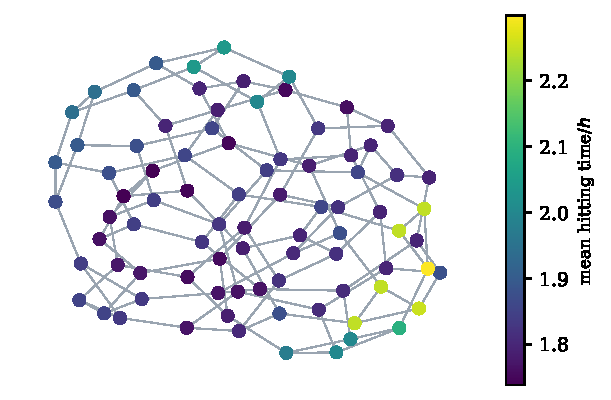
\includegraphics[width=0.7\textwidth]{figs/isogeny.pdf}
\caption{The supersingular $2$ isogeny graph for $N=1009$: $84$ vertices, $3$ regular, without loops or multiple edges. Each vertex $y$ is coloured by $\E_\pi\tau_y/h$, its mean hitting time from a uniformly random start divided by $h$; the average over all $y$ is the Kemeny constant divided by $h$, $1.866$.}\label{fig:08isogeny}
\end{figure}

\section{Random regular graphs}

Alon conjectured that random regular graphs are almost Ramanujan, and Friedman proved it.

\begin{theorem}[Friedman \cite{friedman2008}]
Fix $d\ge3$ and $\varepsilon>0$. With probability tending to one as $n\to\infty$ ($n$ even if $d$ is odd), a uniformly random $d$ regular graph on $n$ vertices has all eigenvalues other than $d$ in $[-2\sqrt{d-1}-\varepsilon,\,2\sqrt{d-1}+\varepsilon]$.
\end{theorem}

Bordenave \cite{bordenave2020} gave a shorter proof through the nonbacktracking matrix $H$ that defines the Ihara zeta function, and extended the theorem to random lifts of a fixed graph. Marcus, Spielman and Srivastava \cite{mss2015,mss2018} proved by interlacing polynomials that bipartite Ramanujan multigraphs exist for every degree and every even number of vertices. Huang, McKenzie and Yau \cite{hmy2024} showed, in a 2024 preprint, that the extreme nontrivial eigenvalues of a random $d$ regular graph fluctuate around $\pm2\sqrt{d-1}$ on the scale $n^{-2/3}$ with the Tracy Widom law of the Gaussian orthogonal ensemble; a consequence is that the probability that a random $d$ regular graph is Ramanujan tends to a constant strictly between $0$ and $1$ (their analysis puts it near $69$ percent). In a computation for this book a random $4$ regular graph on $3000$ vertices had $\lambda_*=3.46376$, just below $2\sqrt3=3.46410$, so that sample is Ramanujan.

\section{Hitting times and Kemeny's constant}\index{Kemeny constant}\index{hitting time}

For simple random walk on $G$ let $h(x,y)=\E_x\tau_y$ with $\tau_y=\min\{t\ge0:X_t=y\}$, as in Appendix~\ref{app:A}; the letter $h$ without arguments keeps its meaning as the number of vertices of an isogeny graph. Kemeny's constant $K=\sum_y\pi(y)h(x,y)$ does not depend on $x$, and for a connected $(q+1)$ regular graph (Theorem~\ref{thm:A:kemeny})
\[
K=\sum_{j\ge2}\frac{1}{1-\lambda_j/(q+1)}=\sum_{t\ge0}\Bigl(\sum_{x}P^t(x,x)-1\Bigr),
\]
where the second form, obtained by expanding each term as a geometric series, requires $G$ not to be bipartite. Since $\pi$ is uniform, $K$ is also the average of $h(x,y)$ over all ordered pairs. The mean hitting time of a fixed target from a uniform start, $\E_\pi\tau_y=n^{-1}\sum_xh(x,y)$, does depend on $y$ (Figure~\ref{fig:08isogeny}); its average over $y$ is $K$.

By the second form, $K/n$ is the expected number of visits to the starting point in excess of equilibrium, averaged over starting points. On the tree the expected number of visits to the start is the Green function $G(1)=q/(q-1)$ of Theorem~\ref{thm:07tree}(5). A graph that looks like a tree from almost every vertex should therefore have $K\approx G(1)\,n$. For isogeny graphs this heuristic is a theorem.

\begin{theorem}[Kemeny constant of isogeny graphs, this book]\label{thm:08kemeny}
Let $\ell$ be prime and let $K_N$ be the Kemeny constant of simple random walk on $G_N(\ell)$, with $h=(N-1)/12$ vertices. As $N\to\infty$ through primes $N\equiv1\bmod12$,
\[
\frac{K_N}{h}\longrightarrow\frac{\ell}{\ell-1}.
\]
Equivalently, the mean hitting time of a uniformly random target, from any fixed start or from a uniformly random one, is asymptotic to $\ell h/(\ell-1)$; for $\ell=2$ it is about $2h$.
\end{theorem}

\begin{proof}
By Theorem~\ref{thm:08brandt} the eigenvalues of the adjacency matrix are $\ell+1$ and $\lambda_j=\sqrt\ell\,x_j$ for $2\le j\le h$, where $x_2,\dots,x_h$ are the normalised eigenvalues of $T_\ell$ on $S_2(\Gamma_0(N))$, counted with multiplicity; by the Ramanujan bound they lie in $[-2,2]$. Since $|\lambda_j|\le2\sqrt\ell<\ell+1$ the graph is connected and not bipartite, and Theorem~\ref{thm:A:kemeny} gives
\[
\frac{K_N}{h}=\frac{h-1}{h}\cdot\frac{1}{h-1}\sum_{j=2}^hg(x_j),\qquad g(x)=\Bigl(1-\frac{\sqrt\ell\,x}{\ell+1}\Bigr)^{-1}.
\]
On $[-2,2]$ we have $\sqrt\ell|x|/(\ell+1)\le\rho_\ell<1$, so $g$ is continuous there, with values in $[1/(1+\rho_\ell),1/(1-\rho_\ell)]$. By the vertical Sato Tate theorem (Theorem~\ref{thm:07serre}, weight $2$, prime level $N\to\infty$, $\ell\nmid N$) the empirical measures $\nu_N=(h-1)^{-1}\sum_{j=2}^h\delta_{x_j}$ converge weakly to the Kesten McKay law $\mu_\ell$. All these measures live on the compact interval $[-2,2]$, where $g$ is continuous, so $\int g\,d\nu_N\to\int g\,d\mu_\ell$, that is,
\[
\frac{1}{h-1}\sum_{j=2}^hg(x_j)\longrightarrow\int_{-2}^2g\,d\mu_\ell .
\]
It remains to evaluate the integral. With $q=\ell$, $g$ is the integrand of the spectral expression for the Green function given after the proof of Theorem~\ref{thm:07tree}, so $\int_{-2}^2g\,d\mu_\ell=G(1)=\ell/(\ell-1)$ by Theorem~\ref{thm:07tree}(5). Since $(h-1)/h\to1$, the theorem follows. The statement about mean hitting times is the identity $K=n^{-2}\sum_{x,y}h(x,y)$ for uniform $\pi$.
\end{proof}

Without the Ramanujan bound the proof would fail: the trivial bound $|x_j|\le(\ell+1)/\sqrt\ell$ does not keep the $x_j$ away from the pole of $g$ at $(\ell+1)/\sqrt\ell$. Chapter~\ref{ch:hit} reads the terms arithmetically. By the Eichler Shimura congruence relation $\prod_{j\ge2}(\ell+1-\lambda_j)=|J_0(N)(\mathbb F_\ell)|$, and $\ell+1-\lambda_j$ is the number of points modulo $\ell$ of an elliptic curve of conductor $N$ when the eigenform has rational coefficients; so $K_N=(\ell+1)\sum_{j\ge2}(\ell+1-\lambda_j)^{-1}$ is a harmonic sum of these factors of $|J_0(N)(\mathbb F_\ell)|$ (Theorem~\ref{thm:hitkemeny}), and $G_N(\ell)$ has $|J_0(N)(\mathbb F_\ell)|/h$ spanning trees, a formula of Hashimoto (Theorem~\ref{thm:hittrees}).

\begin{remark}[An exact series]\label{rem:08exact}
The generating function $\sum_{m\ge0}U_m(x/2)z^m=(1-xz+z^2)^{-1}$ at $z=\ell^{-1/2}$ gives $g(x)=\frac{\ell+1}{\ell}\sum_{m\ge0}\ell^{-m/2}U_m(x/2)$, uniformly on $[-2,2]$ because $|U_m(x/2)|\le m+1$ there. Since $T_\ell T_{\ell^m}=T_{\ell^{m+1}}+\ell T_{\ell^{m-1}}$ on $S_2(\Gamma_0(N))$ for $\ell\nmid N$, as on the tree (Exercise~\ref{ex:07hecke} of Chapter~\ref{ch:07}), the eigenvalue of $T_{\ell^m}$ on the $j$th eigenform is $\ell^{m/2}U_m(x_j/2)$, and therefore
\[
K_N=\frac{\ell+1}{\ell}\sum_{m\ge0}\ell^{-m}\tr\bigl(T_{\ell^m}\mid S_2(\Gamma_0(N))\bigr).
\]
Dividing by $h-1$ and letting $N\to\infty$ term by term (Theorems~\ref{thm:07serre} and~\ref{thm:07tree}(2), with $|U_m(x/2)|\le m+1$) gives, by dominated convergence with the summable bound $(m+1)\ell^{-m/2}$, the limit $\frac{\ell+1}{\ell}\sum_{k\ge0}\ell^{-2k}=\frac{\ell}{\ell-1}$ again. The Eichler Selberg trace formula writes each trace through class numbers, so this series is the natural route to the second order term (Computational Problem~\ref{cp:08second}).
\end{remark}

\subsection{Spectral bounds}

The Ramanujan property also gives uniform bounds valid at every level. Write $\mu_*=\lambda_*/(\ell+1)\le\rho_\ell$, as in Appendix~\ref{app:A}. Since $1/(1+\mu_*)\le1/(1-\mu_j)\le1/(1-\mu_*)$ for $j\ge2$,
\[
\frac{h-1}{1+\rho_\ell}\le K_N\le\frac{h-1}{1-\rho_\ell}.
\]
For individual pairs, with $n=h$, the representation $h(x,y)=n\bigl(Z(y,y)-Z(x,y)\bigr)$ of Appendix~\ref{app:A}, where $\Pi$ is the matrix whose rows all equal $\pi$ and $Z=\sum_t(P^t-\Pi)$, and the bound $|P^t(x,y)-1/n|\le\mu_*^t$ give
\[
\max_{x,y}h(x,y)\le n\sum_{t\ge0}\bigl(|P^t(y,y)-\tfrac1n|+|P^t(x,y)-\tfrac1n|\bigr)\le\frac{2n}{1-\rho_\ell}.
\]
For $\ell=2$ these read $0.51(h-1)\le K_N\le17.5(h-1)$ and $\max h(x,y)\le35h$, while Theorem~\ref{thm:08kemeny} gives $K_N\sim2h$.

\subsection{Data}

For each of the $207$ levels we computed $K_N$ from the spectrum. For $\ell=2$, $K_N/h$ rises from $1.866$ at $h=84$ and lies between $1.971$ and $2.012$ for all $59$ levels with $h\ge500$ (mean $1.988$). For $\ell=3$, $K_N/h$ lies between $1.435$ and $1.515$ throughout, approaching $3/2$. A least squares fit of $a+c/h$ over all levels gives $a=2.004$, $c=-8.2$ for $\ell=2$ and $a=1.498$, $c=-3.0$ for $\ell=3$, consistent with the limits. The scatter about the fit is of the same order as the correction, and it is arithmetic: for $\ell=2$ the mean of $K_N-2h$ is $-3.3$ over the $108$ levels inert in $\Q(\sqrt{-7})$ and $-11.0$ over the other $99$. At the inert levels the curves with complex multiplication by orders of $\Q(\sqrt{-7})$ are supersingular, and the largest single contribution to the difference comes from the one with $j=-3375$ described below. Whether $K_N-2h$ stays bounded is Open Problem~\ref{op:kemeny} of Chapter~\ref{ch:13}. Figure~\ref{fig:08kemeny} shows the convergence.

As an independent check we solved the hitting time equations directly for every target on $G_N(2)$ for $N=1009,2017,4129$ ($h=84,168,344$). The Kemeny constants are $156.766$, $324.736$ and $682.586$, so that $K_N/h=1.866$, $1.933$, $1.984$, and they agree with the spectral formula to a relative error below $10^{-13}$. The maximal hitting times divided by $h$ are $2.58$, $3.35$ and $5.98$, far below the bound $35$; they reflect the neighbourhood of the hardest target, not growth in $h$. At $N=4129$ that target is the curve with $j=-3375$, which has complex multiplication by the maximal order of $\Q(\sqrt{-7})$ and is supersingular because $4129$ is inert in that field. Its endomorphisms $(1\pm\sqrt{-7})/2$ of degree $2$ form a loop counted twice, so the walk stays put with probability $2/3$. If the rest of its neighbourhood is a tree, a walk started there returns with probability $\frac23+\frac13\cdot\frac12=\frac56$ and makes $6$ visits on average, against $G(1)=2$ at a vertex whose neighbourhood is a tree, so its mean hitting time is about $6h$ (Exercise~\ref{ex:08target}). At $N=2017$ the hardest targets are the two curves with complex multiplication by the maximal order of $\Q(\sqrt{-15})$, which are joined by a double edge.

\begin{figure}[t]\centering
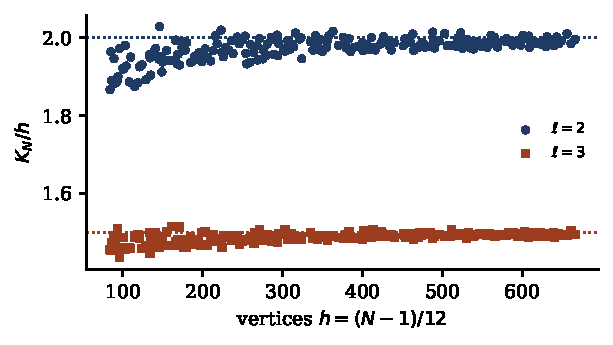
\includegraphics[width=0.75\textwidth]{figs/kemeny.pdf}
\caption{Kemeny constants $K_N$ of the supersingular $\ell$ isogeny graphs for $\ell=2,3$ at the $207$ primes $N\equiv1\bmod12$ between $1000$ and $8000$, divided by the number of vertices $h=(N-1)/12$, against the limits $2$ ($\ell=2$) and $3/2$ ($\ell=3$) of Theorem~\ref{thm:08kemeny} (dotted lines).}\label{fig:08kemeny}
\end{figure}

\section{Isogeny graphs in cryptography}

Charles, Goren and Lauter \cite{cgl2009} proposed a hash function built from walks on $G_N(2)$: the bits of the message choose, at each step, one of the two edges that do not backtrack, starting from a fixed curve, and the hash value is the endpoint. Because the graph is Ramanujan, a walk of $O(\log N)$ steps ends at a nearly uniform vertex. A collision gives two distinct paths between the same curves, hence a cycle and an endomorphism of the starting curve that is not multiplication by an integer, so security rests on the presumed difficulty of finding paths in the graph. Under the generalized Riemann hypothesis this problem is equivalent to computing endomorphism rings of supersingular curves \cite{wesolowski2022}. All known classical algorithms for it take time exponential in $\log N$; the method of Delfs and Galbraith \cite{delfsgalbraith2016} takes about $\sqrt N$ steps up to logarithmic factors. We make no claim about particular schemes and note only that the key exchange SIDH of Jao and De Feo \cite{jaodefeo2011}, which also publishes the images of torsion points under the secret isogeny, was broken in 2022 by an attack that exploits this extra information and does not solve the general path problem \cite{castryckdecru2023}. Theorem~\ref{thm:08kemeny} quantifies the cost of naive search: from any fixed start, a random walk looking for a target curve chosen uniformly at random needs $K_N\approx2h\approx N/6$ steps on average, far more than $\sqrt N$.

\section{Notes}

Ihara's zeta function appeared in his work on discrete subgroups of $p$ adic groups \cite{ihara1966}; Serre's book \cite{serre1980} made the link with graphs explicit, Sunada \cite{sunada1986} suggested general graphs, and Hashimoto \cite{hashimoto1989} and Bass \cite{bass1992} proved the determinant formula in general. Terras's book \cite{terras2011} is an introduction. The equivalence of the graph Riemann hypothesis and the Ramanujan property is standard; the third form in Proposition~\ref{prop:08three} is a reformulation we find useful because it ties the Riemann hypothesis to the Kesten rate. Supersingular graphs go back to Deuring, Eichler and Mestre \cite{mestre1986}; Pizer \cite{pizer1990} identified them as Ramanujan graphs, and Gross \cite{gross1987} used Brandt matrices for special values of $L$ functions. Kemeny and Snell \cite{kemenysnell1960} introduced the constant that bears Kemeny's name. Theorem~\ref{thm:08kemeny} is new as far as we know; it is a direct consequence of Serre's theorem once the Kemeny constant is recognised as a spectral statistic whose tree value is the gambler's ruin constant. The same constant appears for random regular graphs: Cooper and Frieze \cite{cooperfrieze2005} proved that the cover time of a random $r$ regular graph is asymptotic to $\frac{r-1}{r-2}\,n\log n$, through hitting times of order $\frac{r-1}{r-2}\,n$ at vertices whose neighbourhoods are trees, and $\frac{r-1}{r-2}=\frac{\ell}{\ell-1}$ when $r=\ell+1$.

\section{Exercises}

\begin{enumerate}
\item Prove that $u\,Z_G'(u)/Z_G(u)=\sum_mN_mu^m$. For a $(q+1)$ regular graph deduce from the Ihara Bass formula that $N_m=\sum_j(\alpha_j^m+\beta_j^m)+(|E|-n)(1+(-1)^m)$, where $\alpha_j,\beta_j$ are the roots of $t^2-\lambda_jt+q$.
\item For the complete graph on $q+2$ vertices compute $Z_G$, verify the graph Riemann hypothesis, and check $K=(n-1)^2/n$.
\item Show that a connected $(q+1)$ regular graph with $q\ge2$ is bipartite if and only if $-(q+1)$ is an eigenvalue, and that $u=-1/q$ is a pole of $Z_G$ exactly in that case. Find the order of the pole of $Z_G$ at $u=-1$ in both cases.
\item\label{ex:08alon} Prove the Alon Boppana bound in the weak form $\liminf\lambda_*\ge2\sqrt q$ for a sequence of $(q+1)$ regular graphs with $n\to\infty$. (Hint: by the recursions of Theorem~\ref{thm:07tree}(1), which hold on any $(q+1)$ regular graph, $A^{2k}$ is a combination with nonnegative coefficients of the nonbacktracking matrices $A_m$, whose traces are nonnegative, and the coefficient of $A_0=I$ is the number $q^k\int x^{2k}\,d\mu_q$ of closed walks of length $2k$ at a vertex of the tree. Compare with $\tr A^{2k}\le2(q+1)^{2k}+n\lambda_*^{2k}$, which allows for a bipartite graph, and let $k\to\infty$ slowly with $n$.)
\item\label{ex:08target} Show that for every target $y$, $\E_\pi\tau_y=\frac1n\sum_xh(x,y)=n\,Z(y,y)$, and interpret $Z(y,y)$ as an excess number of visits. For $q=2$, compute the expected number of visits to $y$ of simple random walk started at $y$ on an infinite $3$ regular graph that is a tree except that $y$ carries a loop counted twice, and compare with $G(1)=2$ and with the hardest target at $N=4129$. Do the same when $y$ carries a half loop instead, and when $y$ is joined to a neighbour by a double edge (answers $6$, $3$ and $10/3$).
\end{enumerate}

\section{Open computational problems}

\begin{compproblem}[Second order term of the Kemeny constant]\label{cp:08second}
Objective: determine the correction $K_N-\ell h/(\ell-1)$ as a function of $N$. Data: all primes $N\equiv1\bmod12$ up to $10^6$, $\ell=2,3$. Algorithm: the series of Remark~\ref{rem:08exact}, with $\tr T_{\ell^m}$ from the Eichler Selberg trace formula, whose elliptic term is a sum of Hurwitz class numbers $H(4\ell^m-s^2)$ weighted by Legendre symbols at $N$ and whose identity, hyperbolic and weight two divisor terms are explicit (the identity term, $(N+1)/12$ for even $m$, contributes $\ell/(6(\ell-1))$ to the correction); the class numbers do not depend on $N$ and can be tabulated once, and the series is truncated at $m$ of order $\log N$. Check against PARI/GP spectra for $N\le10^5$. Deliverable: the empirical law of the correction, its regression on the symbols $(D/N)$ for small discriminants $D$, and a conjectural formula in terms of class numbers. Why it matters: the correction is where the elliptic terms, invisible in the limit, become measurable; it explains the scatter in Figure~\ref{fig:08kemeny}, which for $\ell=2$ is led by $D=-7$, and it is the computational side of Open Problem~\ref{op:kemeny} of Chapter~\ref{ch:13}.
\end{compproblem}

\begin{compproblem}[Hitting times on large supersingular graphs]
Objective: the distribution over targets $y$ of the mean hitting time $\E_\pi\tau_y/h=Z(y,y)$ on $G_N(2)$, and of $\max_{x,y}h(x,y)/h$, which the spectral bound keeps below $35$. Data: $G_N(2)$ for $N$ up to $10^7$ ($h$ near $8\times10^5$), walks generated on the fly from $\Phi_2$ over $\mathbb F_{N^2}$. Algorithm: $10^5$ Monte Carlo walks per level on GPU, run in continuous time with exponential holding times of mean one, which leaves the means unchanged, with exact sparse solves for $N\le10^5$ as ground truth. Deliverable: histograms of $\E_\pi\tau_y/h$ over targets, with the atoms predicted by Exercise~\ref{ex:08target}, and the law of $\tau_y/\E_\pi\tau_y$ against the exponential law that Corollary~\ref{cor:10cisogeny} of Chapter~\ref{ch:10c} guarantees up to $O(1/h)$. Why it matters: the exponential law predicts the cost of naive search once the mean is known, and the means carry the arithmetic, through curves with complex multiplication by small discriminants.
\end{compproblem}

\begin{compproblem}[Other degrees and ordinary curves]
Objective: repeat the analysis for $\ell=5,7$ and for $\ell$ isogeny graphs of ordinary curves. Data: supersingular $G_N(\ell)$ for $N\le10^5$; ordinary isogeny volcanoes over $\mathbb F_N$ for $N\le10^6$ (Sutherland's algorithms or Sage). Deliverable: $K_N/h$ against $\ell/(\ell-1)$, and for volcanoes the Kemeny constant as a function of the class group and the depth. Why it matters: volcanoes are governed by class groups of imaginary quadratic orders rather than by the Ramanujan bound, so the comparison isolates what Theorem~\ref{thm:08kemeny} owes to the Ramanujan property.
\end{compproblem}

\begin{compproblem}[Ihara zeta as a test for random lifts]
Objective: the probability that a random $k$ fold lift of $G_N(2)$ satisfies the graph Riemann hypothesis for its new poles. Data: lifts of index $k\le100$ of graphs with $h\le500$, $10^4$ lifts each. Algorithm: largest new eigenvalue of the nonbacktracking matrix $H$ by sparse Arnoldi iteration. Deliverable: the empirical probability as a function of $k$ and $h$, with Tracy Widom fits at the edge. Why it matters: Bordenave proved that random lifts are almost Ramanujan; whether lifts of arithmetic graphs behave like random graphs probes how much arithmetic survives a random perturbation.
\end{compproblem}
